\documentclass{article}
\usepackage[utf8]{inputenc}
\usepackage{hyperref}



\title{Généralités réseaux de neurones et deep-learning}
%\author{alice.lasserre }
\date{June 2021}

\usepackage{natbib}
\usepackage{graphicx}
\usepackage{graphicx}
\usepackage{fullpage}
\usepackage{eso-pic}
\usepackage{listings}
\usepackage{ulem}
\usepackage{float}
\usepackage{comment}


\begin{document}

\maketitle



Durée : 25 mn

\section{Prérequis}

\begin{itemize}
\item Notions de programmation et d'algorithmique primaires
\end{itemize}


\section{Acquis d'apprentissage}

\begin{itemize}
\item Notions de construction de neurones et réseaux denses
\end{itemize}


\begin{figure}[H]
\begin{minipage}[c]{0.4\linewidth}

\centering
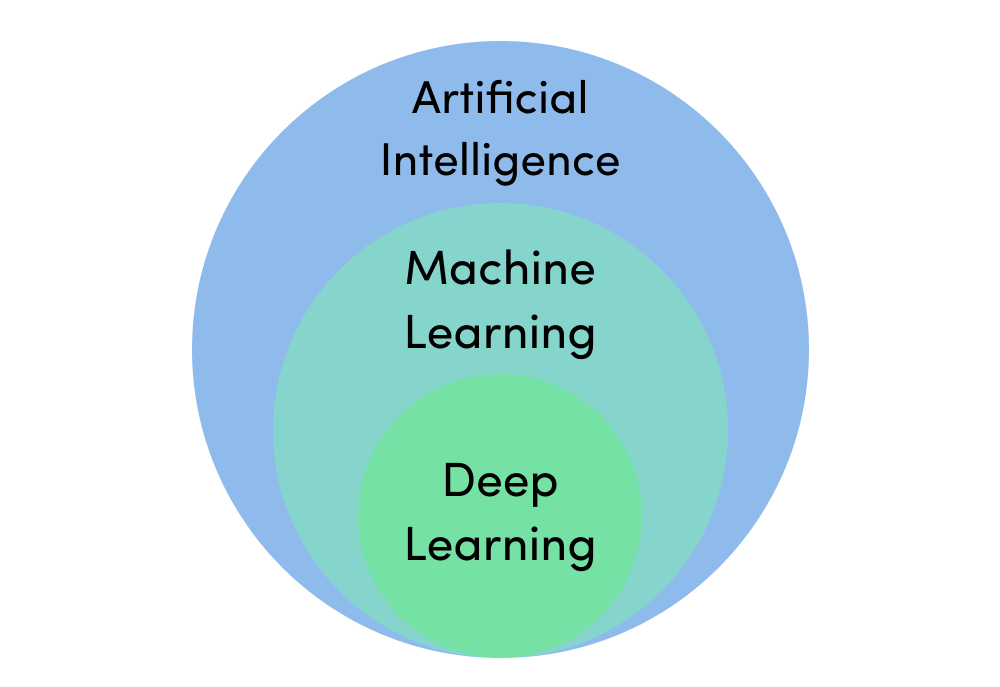
\includegraphics[width=0.8\textwidth]{img/diagram1.png}
https://levity.ai/blog/difference-machine-learning-deep-learning

\end{minipage} \hfill
\begin{minipage}[c]{0.6\linewidth}


Le terme d'\textbf{intelligence artificielle} définit l'ensemble des théories et des techniques 
mises en œuvre en vue de réaliser des machines capables de mimer le fonctionnement du cerveau humain, 
ou du moins sa logique lorsqu’il s’agit de prendre des décisions. \\

Le terme de \textbf{machine learning} désigne une sous-branche de l'intelligence artificielle.
Il inclut des techniques qui permettent aux machines d'améliorer leurs performances par apprentissage.
Il existe deux types d'apprentissage : l'\textit{apprentissage supervisé} et \textit{non-supervisé}.
\begin{itemize}
\item L'\textit{apprentissage supervisé} correspond à un réseau où chaque données d'entraînements est attachée à un label. 
Ce dernier correspond à la réponse que l'algorithme doit trouver. 
\item L'\textit{apprentissage non supervisé} correspond à un réseau où les données d'entraînements ne sont pas étiquetées.
L'algorithme ne peut donc pas vérifier l'exactitude de ses réponses.

\end{itemize}

Le terme de \textbf{deep learning} désigne une sous-branche de machine learning. 
Il est basé sur des réseaux de neurones qui permettent à la machine de 
s'entraîner pour réaliser une certaines tâche. Les réseaux profonds utilisent 
plusieurs couches de neurones (couches cachées). 

\end{minipage}
\end{figure}


\section{Réseaux de neurones}

\subsection{Le neurone artificiel}

C'est une unité de traitement informatique qui reçoit des entrées $x_i$ affectées chacune d'un poids $\omega_i$. 
La sortie du neurone est donnée par la valeur de sa \textbf{fonction d'activation} en un point défini par la 
\textbf{combinaison linéaire de ses entrées} $\sum_i \omega_i x_i - b$ :

\begin{figure}[H]
\centering
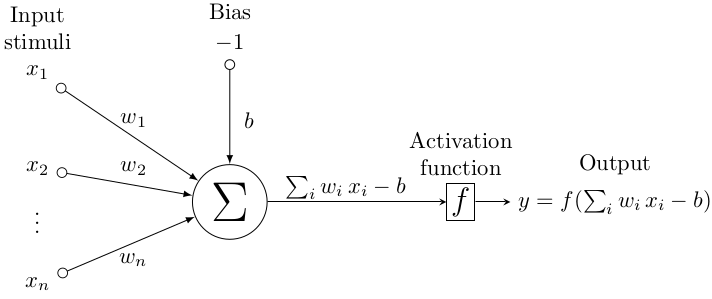
\includegraphics[width=0.8\textwidth]{img/nn_1.png}
JLC
\end{figure}


L'entrée \textit{Bias} (b) reçoit le stimuli "-1" affecté du poids $b$ : 
il permet de décaler le point où la fonction d'activation est calculée. 

\subsection{Fonction d'activation}

La fonction d'activation permet de calculer la sortie d'un neurone artificiel.\\

Principaux rôles :

\begin{itemize}
\item introduire dans le neurone un comportement \textbf{non linéaire} (comme des mécanismes de seuil, de saturation...)
\item fixer la plage de sortie de la valeur calculée par le neurone, par exemple dans l'intervalle $[-1 ; 1]$, $[0 ; 1]$ ou encore $[0 ; +\infty[$
\end{itemize}

Exemples de fonctions d'activations couramment utilisées :

\begin{figure}[H]
\centering
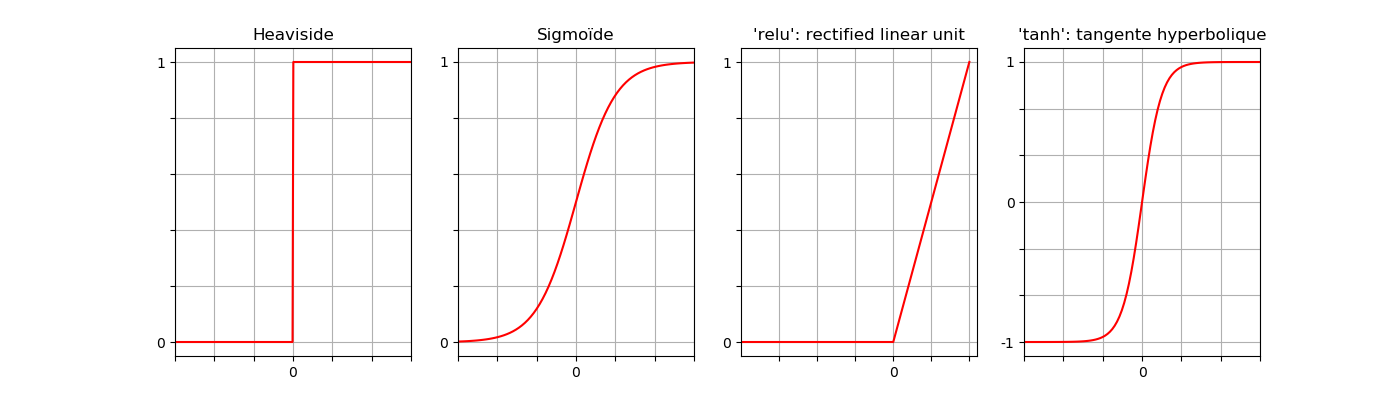
\includegraphics[width=1\textwidth]{img/activationFunctions.png}
JLC
\end{figure}

\subsection{Réseau dense séquentiel}

Pour créer un réseau de neurones dense séquentiel on connecte les sorties 
des neurones d'une couche sur les entrées des neurones de la couche suivante. 
Chaque neurone possède ses propres poids et son propre biais. 
On peut voir chaque neuronne comme une fonction : 
il prend toutes les sorties de la couche précédente 
puis il calcule et renvoit la valeur de sa fonction d'activation.

\bigskip

L'image ci-dessous présente un \textbf{réseau dense séquentiel}, avec :

\begin{itemize}

\item une \textbf{couche d'entrée} de 784 valeurs comprises entre 0 et 1 (les pixels des 
images MNIST 28 $\times$ 28 mis sous forme d'un vecteur de 784 nombres `float`),

\item une \textbf{couche cachée} de 784 neurones utilisant la fonction d'activation `relu`,

\item une \textbf{couche de sortie} à 10 neurones, pour la classification des images en 10 
classes associées aux chiffres {0,1,2...9}, utilisant la fonction d'activation 
`softmax` adaptée aux problèmes de classification.

\end{itemize}

\begin{figure}[H]
\centering
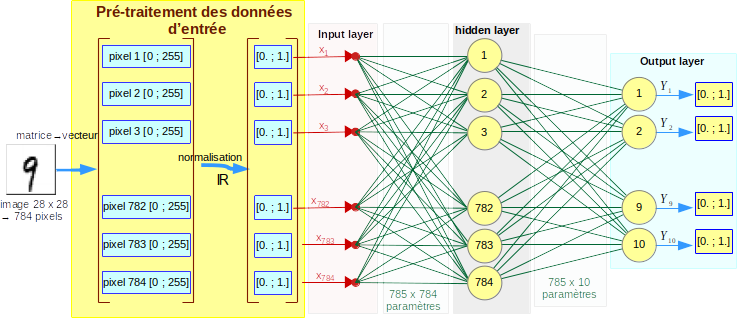
\includegraphics[width=1\textwidth]{img/archiReseau.png}
JLC
\end{figure}

Remarques : 

\begin{itemize}
\item Chaque neurone de la première couche cachée reçoit 785 entrées : les 784 valeurs $x_i$ des pixels de l'image plus le biais (l'entrée '-1'). 
\item Il y a donc 785 inconnues pour chaque neurone : les 784 poids $w_i$ affectés à chaque entrée $x_i$, plus le  poids $b$ affecté au biais.
\item On compte donc 785 $\times$ 784 inconnues pour la couche cachée et 785 $\times$ 10 inconnues pour la couche de sortie : 
soit un total de 623290 inconnues dont la valeur doit être optimisée par l'algorithme d'apprentissage du réseau.
\end{itemize}



\subsection{Intérêt de la fonction d'activation softmax pour les problèmes de classification}

Dans les problèmes de classification, on a besoin que les sorties de la dernière couche 
puissent servir à décider quelle est la classe reconnue par le réseau pour une enrée donnée.
Une solution est de transformer les sorties des neurones de la dernière couche en probabilités, 
en utilisant la fonction d'activation \textbf{Softmax}. On obtient alors une distribution de probabilité : 
la somme de toutes les sorties est égale à 1.


\bigskip



La fonction `softmax` calcule pour chaque neurone de sortie $k$ la valeur $\displaystyle{Y_k = \frac{e^{y_k}}{\sum_i{e^{y_i}}}}$,
où $y_k$ désigne la combinaison linéaire $\sum_i \omega_i x_i - b$ calculée par le neurone $k$.


\bigskip


`softmax` associe ainsi à chacune des sorties $y_k$ une valeur $Y_k \in [0, 1]$ 
qui peut être interprétée comme la probablité de la sortie $k$ : 
on obtient une valeur proche de 1 pour le neurone fournissant 
la valeur $y_i$ la plus grande, et quasiment 0 pour tous les autres.

\begin{figure}[H]
\centering
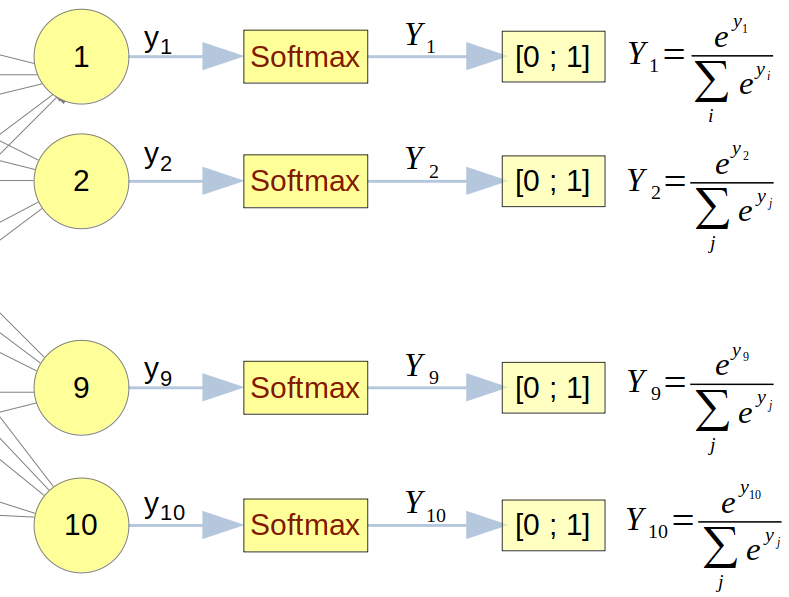
\includegraphics[width=0.7\textwidth]{img/softmax.png}
JLC
\end{figure}


\subsection{Catégorisation des labels (\textbf{one-hot coding})}

Dans les problèmes d'entraînement supervisé, les classes à reconnaître sont identifiées
par une étiquette "lisible" par l'être humain ("chien", "vélo", "personne"...), 
présentée au réseau de neurones sous la forme d'un entier (le numéro de classe: "chien" $\rightarrow$ 1, "vélo $\rightarrow$ 2...). 
La comparaison des sorties du réseau de neurones (liste de probabilités) avec 
l'entier désignant la classe n'est pas directe... 
Pour faciliter la comparaison entre l'entier désignant une clase à reconnaître et les probabilités 
calculées par le réseau sur ses neurones de sortie, on utilise la technique de \textbf{catégorisation} qui associe 
à un entier un vecteur dont les éléments sont tous nuls sauf un (one-hot coding).



\newpage




Par exemple pour un problème de classification à 10 classes la représentation one-hot coded donne : \\


\begin{tabular}{|l|c|r|}
  \hline
  chiffre &  $Y^\prime\_i$ : vecteur \textit{one-hot} \\
  \hline
  0 & [1 0 0 0 0 0 0 0 0 0]\\
  1 & [0 1 0 0 0 0 0 0 0 0]\\
  2 & [0 0 1 0 0 0 0 0 0 0]\\
  3 & [0 0 0 1 0 0 0 0 0 0]\\
  4 & [0 0 0 0 1 0 0 0 0 0]\\
  5 & [0 0 0 0 0 1 0 0 0 0]\\
  6 & [0 0 0 0 0 0 1 0 0 0]\\
  7 & [0 0 0 0 0 0 0 1 0 0]\\
  8 & [0 0 0 0 0 0 0 0 1 0]\\
  9 & [0 0 0 0 0 0 0 0 0 1]\\
  \hline
\end{tabular}

\subsection{Calcul de l'erreur d'inférence du réseau}

Dans les problèmes d'\textbf{entraînement supervisé}, on doit calculer l'erreur d'inférence 
du réseau lorsqu'on l'entraîne avec des données labellisées. 
Cette erreur sert à modifier les poids du réseau grâce à l'algorithme de \textit{back propagation}. 

On définit une fonction de perte (\textit{loss function}) qui permet de calculer l'écart entre 
l'inférence du réseau de neurones et le résultat attendu. 
Le but de l'apprentissage est de modifier les poids du réseau 
de neurones pour minimiser cette fonction de perte.

Dans les problèmes de \textbf{classification} où l'inférebce du réseau se présente 
sous la forme d'un vectuer de probabiltés, on peut utiliser l'erreur \textit{cross entropy}
($-\sum_i{Y'_i.\log{Y_i}}$) qui mesure l'écart entre la représentation 
\textit{one-hot} du label et la réponse du réseau :


\begin{figure}[H]
\centering
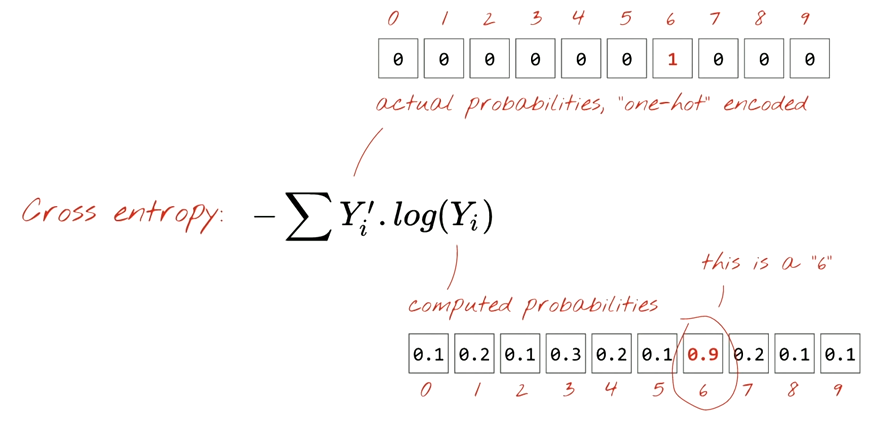
\includegraphics[width=1\textwidth]{img/CrossEntropy.png}

\medskip
vidéo "Deep Learning TensorFlow" de Martin Gorner
\end{figure}


\subsection{Backpropagation error}

L'algorithme de \textbf{rétropropagation de l'erreur} permet de modifier les poids 
des neurones du réseau pour minimiser l'erreur entre valeur attendue et 
valeur prédite par le réseau. 
Au fur et à mesure des apprentissages successifs, les poids du réseau convergent 
vers un état qui minimize l'erreur d'inférence du réseau et qui constitue
 l'état du réseau entraîné.

On initialise le réseau avec des poids et des biais aléatoires pour chaque neurone
et on les ajuste au fur et à mesure de l'entraînement. 
Lorsque le réseau est peu ou pas entrainé, les sorties du réseau sont loin des sorties attendues. 

Les données d'entrée du réseau sont regroupées en paquets (\textbf{batch}) : 
chaque paquet fait l'objet d'entraînements successifs qui permettent 
d'améliorer la minimisation de la fonction d'erreur. 
Le nombre d'entraînements du réseau sur un même batch est 
appelé "nombre d'époques" (\textbf{n\_epochs}).

\subsection{Optimiseur}

La recherche du minimum de la fonction d'erreur est confié à un \textbf{optimiseur} :  
un des algorithmes les plus simples est la \textit{descente de gradient} (GD), 
qui consiste à se déplacer dans le sens de la pente la plus forte à chaque itération d'entraînement.

\textbf{Adam} est un optimiseur plus complexe que \textbf{GD}. Sur l'animation ci-dessous on voit 
plusieurs optimiseurs se déplacer sur une fonction de coût ne comportant que 2 paramètres
 (au lieu de plusieurs milliers...) à la recherche d'un minimum. 


\bigskip
(Numbers in figure legend indicate learning rate, specific to each Optimizer.)
Tu peux télécharger l'animation en cliquant \href{https://github.com/Jaewan-Yun/optimizer-visualization/raw/master/figures/movie11.gif}{ici}.


Une autre caracteristique de l'algorithme GD, est que le pas effectué à chaque itération est fixe. 
L'image suivante montre Adam et GD dans un cas ou la pente devient très forte :

Tu peux télécharger l'animation en cliquant \href{https://github.com/Jaewan-Yun/optimizer-visualization/raw/master/figures/movie9.gif}{ici}.

\end{document}
